%!TeX  root  =  user_guide.tex

\chapter{Using QGIS Core Plugins}\label{sec:core_plugins}\index{plugins!core}

% when the revision of a section has been finalized, 
% comment out the following line:
% \updatedisclaimer

{\setlength{\extrarowheight}{15pt}
\small
\begin{longtable}{|p{1.2cm}|p{3.8cm}|p{7.5cm}|p{3cm}|}
\caption{26 QGIS Core Plugins}\label{tab:core_plugins} \\
\hline
 \textbf{Icon} & \textbf{Plugin} & \textbf{Description} & \textbf{Manual Reference}\\
\endfirsthead
\hline
\textbf{Icon} & \textbf{Plugin} & \textbf{Description} & \textbf{Manual Reference}\\
\endhead
\hline

\includegraphics[width=0.6cm]{delimited_text}
 & Add Delimited Text Layer \index{plugins!delimited text} & Loads and displays delimited text files containing x,y coordinates & Chapter \ref{label_dltext}\\
\hline

\includegraphics[width=0.6cm]{coordinate_capture}
 & Coordinate Capture \index{plugins!coordinate capture}& Capture mouse coordinate in different CRS & Chapter \ref{coordcapt}\\
\hline 

\includegraphics[width=0.6cm]{copyright_label}
 & Copyright Label \index{plugins!copyright}& Draws a copyright label with information & Chapter \ref{copyrightlabel}\\
\hline

\includegraphics[width=0.6cm]{plugin}
 & Diagram Overlay \index{plugins!diagram}& Placing diagrams on vector layers & Chapter \ref{sec:diagram}\\
\hline

\includegraphics[width=0.6cm]{plugin}
 & Displacement plugin \index{plugins!point displacement}& Add new renderer that automatically handles point displacement in case they have the same position & Chapter \ref{new_generation_sym}\\
\hline
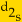
\includegraphics[width=0.6cm]{dxf2shp_converter}
 & DXF2Shape Converter \index{plugins!DXF2Shape}& Converts from DXF to SHP file format & Chapter \ref{dxf2shape}\\
\hline

\includegraphics[width=0.6cm]{plugin}
 & eVis & Event Visualization Tool & Chapter \ref{sec:evis}\\
\hline

\includegraphics[width=0.6cm, height=0.6cm]{ftools_logo}
 & fTools \index{plugins!ftools}& A suite of analysis, geometry, geoprocessing, and research tools & Chapter \ref{sec:ftools}\\
\hline

\includegraphics[width=0.6cm]{gps_importer}
 & GPS Tools \index{plugins!gps}& Tools for loading and importing GPS data & Chapter \ref{label_plugingps}\\
\hline

\includegraphics[width=0.6cm]{grass}
 & GRASS \index{plugin!grass toolbox} & Activates the mighty GRASS Toolbox & Chapter \ref{sec:grass}\\
\hline

\includegraphics[width=0.6cm, height=0.6cm]{raster-info}
 & GDAL Tools \index{plugins!gdaltools} & Raster tools: simplified graphical interface for most commonly used programs & Chapter \ref{label_plugingdaltools}\\
\hline

\includegraphics[width=0.6cm]{georeferencer}
 & Georeferencer GDAL \index{plugin!georeferencer} & Adding projection info to Rasterfiles using GDAL & Chapter \ref{sec:georef}\\
\hline

\includegraphics[width=0.6cm]{interpolation}
& Interpolation plugin \index{plugins!Interpolation}& Interpolation on base of vertices of a vector layer & Chapter \ref{sec:interpol}\\
\hline

\includegraphics[width=0.6cm]{mapserver_export}
& MapServer Export Plugin \index{plugins!MapServer Export}& Export a saved QGIS project file to a MapServer map file & Chapter \ref{sec:mapserver_export} \\
\hline

\includegraphics[width=0.6cm]{north_arrow}
& North Arrow \index{plugins!north arrow}& Displays a north arrow overlayed onto the map & Chapter \ref{northarrow}\\
\hline

\includegraphics[width=0.6cm]{offline_editing_copy}
 & Offline Editing & Offline editing and synchronizing with database & Chapter \ref{sec:offlinedit}\\
\hline
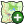
\includegraphics[width=0.6cm]{osm_load}
 & OpenStreetMap & Visualize and edit OpenStreetMap data & Chapter \ref{plugins_osm}\\
\hline

\includegraphics[width=0.6cm]{oracle_raster}
 & Oracle Spatial Georaster \index{plugins!georaster}& Access Oracle Spatial GeoRasters & Chapter 
\ref{sec:oracleraster}\\
\hline
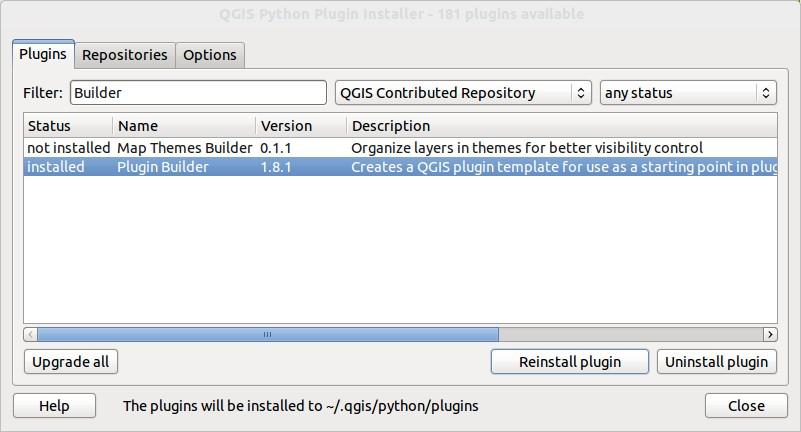
\includegraphics[width=0.6cm]{plugin_installer}
 & Plugin Installer \index{plugins!Plugin Installer} & Download and install python plugins & Chapter \ref{sec:python_plugin_installer}\\
\hline

\includegraphics[width=0.6cm]{raster_terrain}
& Raster Terrain Modelling \index{plugins!Raster Terrain Modelling}& Compute slope, aspect,
ruggedness and total curvature of DEMs & Chapter \ref{sec:rasterrain}\\
\hline

\includegraphics[width=0.6cm]{plugin}
 & Road graph Plugin \index{plugins!road graph} & Solve shortest path problem & Chapter \ref{sec:roadgraph} \\
\hline

\includegraphics[width=0.6cm]{spiticon}
 & SPIT \index{plugins!spit} & Shapefile to Postgres/PostGIS Import Tool & Chapter \ref{sec:loading_postgis_data} \\
 \hline

\includegraphics[width=0.6cm]{plugin}
 & SQL Anywhere plugin \index{plugins!SQL anywhere} &  Store vector layers 
within a SQL anywhere database & Chapter \ref{sec:sqlanywhere} \\
 \hline

\includegraphics[width=0.6cm]{scale_bar}
 & Scalebar \index{plugins!scalebar}& Draws a scale bar & Chapter \ref{scalebar} \\
\hline

\includegraphics[width=0.6cm]{spatialquery}
 & Spatial Query & Make spatial queries on vector layers & Chapter \ref{sec:spatial_query} \\
\hline

\includegraphics[width=0.6cm]{mIconAddWfsLayer}
 & WFS Plugin & Add WFS layers to the QGIS canvas & Chapter \ref{sec:ogc-wfs} \\
\hline
\end{longtable}}

\newpage

